\documentclass[a4paper, 11pt]{article}

\usepackage[utf8]{inputenc}
\usepackage[french]{babel}
\usepackage{graphicx}

\title{INFOB317 : Projet Tour de France}
\author{BERG Thibaut - GAILLARD Matthys - SANTELÉ Victor - SMITH Jonathan}

\begin{document}

\maketitle

\newpage

\section{Introduction}

Dans le cadre du cours INFOB317 : Intelligence artificielle et programmation symbolique, nous avons été amenés à informatiser le jeu du Tour de France en une interface web grâce à React et à y ajouter des fonctionnalités intelligente comme un ChatBot auquel on peut poser des questions ou encore une intelligence artificielle jouant le rôle d'adversaire.\newline

Ce projet a été divisé en trois grandes parties :
\begin{itemize}
    \item La conception du jeu et de ses mécaniques
    \item La conception du ChatBot
    \item La conception de l'intelligence artificielle adverse\newline
\end{itemize}

Il est évident de préciser que le projet se base principalement sur la conception du jeu et de ses mécaniques. Dessus, nous avons implémenté le ChatBot et l'intelligence artificielle adversaire. Ce rapport a pour but de décrire la construction du projet et les techniques mises en place. Celui-ci se déroulera en plusieurs parties : 

\begin{enumerate}
	\item \textbf{Démarche générale} : décrit la démarche générale du groupe sur la réalisation du projet et les décisions qui ont été prisent concernant l'implémentation du jeu.
	\item \textbf{Outils} : présente les outils que nous avons utilisés pour mener à bien le projet et donne les raisons de nos choix.
	\item \textbf{Mécaniques de jeu} : décortique comment nous avons construit la structure du jeu et comment nous avons représenté et implémenté le jeu et ses règles en informatique.
	\item \textbf{ChatBot explicateur} : décrit la construction du ChatBot et apporte des informations concernant certaines de ses particularités.
	\item \textbf{Interface} : décrit la construction de l'interface web du jeu et son organisation.
	\item \textbf{Intelligence artificielle adversaire} : décrit la construction de l'intelligence artificielle que le joueur va combattre et son fonctionnement.\newline
\end{enumerate}

Enfin, comme pour tout rapport, nous terminerons par une conclusion dans laquelle nous expliquerons notre ressenti par rapport au projet. Nous expliciterons ce que nous avons trouvé comme points forts et points faibles du projet. Nous aborderons également des pistes pour améliorer le projet.

\newpage

\section{Démarche générale}

Cette partie est consacrée à la démarche que nous avons suivie lors de la réalisation du jeu.\newline

Dès le départ, nous avons choisi de diviser le travail par fonctionnalités. Il fallait établir comment nous allions structurer le projet et comment représenter le jeu en code informatique. Il y a donc une des personnes du groupe qui s'est concentrée sur la création du jeu et de ses mécaniques après avoir définit la structure du programme. Rapidement, une autre personne du groupe l'a aidé et ils ont travaillé en binôme. Cependant, afin de voir le rendu de ces implémentations, ils ont du travaillé sur l'interface en même temps. Pendant ce temps, une troisième personne s'est chargée d'alimenter le ChatBot afin qu'il puisse répondre aux questions des joueurs. Enfin, les deux personnes chargées des mécaniques de jeu ont travaillé en parallèle sur l'intelligence artificielle adversaire.\newline

Concernant le choix des outils, il a principalement été fait par la première personne en charge des mécaniques de jeu. Cette même personne a choisit la réelle architecture du projet et son binôme l'a aidé à peaufiner les détails l'architecture.

\section{Outils}

Nous avons choisi d'utiliser React comme base pour construire le site web et le projet. Il s'agit donc ici d'une single-page application. Cependant, toute l'intelligence du projet est écrit en Prolog. La partie React et donc TypeScript sert juste d'interface entre les states envoyés et reçus.\newline

Évidemment, le jeu fonctionne grâce à des requêtes HTTP et la communication pour le chat se fait via WebSocket. Enfin, nous avons décidé de déployé le projet sur Azure Container App et Azure Static Web App. 

\newpage

\section{Mécaniques de jeu}

\newpage

\section{ChatBot explicateur}

Pour la construction du ChatBot, nous l'avons alimenté de 61 questions et nous avons ajouté des filtres permettant à celui-ci de mieux interpréter les questions posées par les utilisateurs. Les 61 questions couvrent la totalité des subtilités du jeu et permettent aux joueurs un peu perdus d'être guidé afin de mieux aborder le jeu.\newline

Toutes les questions ont été structurées afin que le bot reconnaisse seulement les mots importants de la phrase. Grâce à ça, le bot est très tolérant dans la compréhension des différents styles de questions qu'un joueur peut poser. Cette structure ressemble à ceci : 

\begin{figure}[!h]
	\centering
	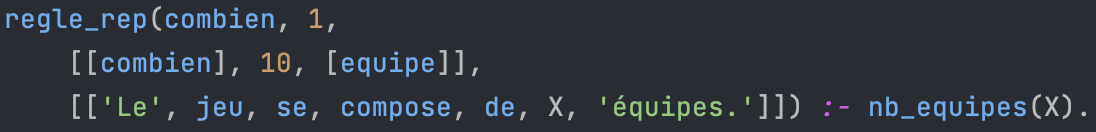
\includegraphics[scale=.6]{assets/question-structure.png}
	\caption{Structure des questions}
\end{figure}

Cette structure permet de demander au bot de reconnaître le mot "combien" suivit de mots avant de voir le mot "equipe". Il faut préciser que le nombre de mots entre les mots "combien" et "equipe" doivent être entre 0 et 10.\newline

Il faut préciser qu'un des gros problèmes dans la création d'un bot en français est la gestion des accents. En informatique, la lettre "e" et la lettre "é" ne correspondent pas au même code. Il a donc fallut ajouter un filtre permettant de retirer ces accents au cas où le joueur mettrait des accents dans sa question. Il est possible que celui-ci en mette ou n'en mette pas. Afin de ne pas frustrer le joueur, il faut que le bot puisse comprendre les différentes situations.\newline

Nous avons donc décidé que toutes les questions que le bot comprenne ne possèdent aucun accent. Afin de permettre que cela fonctionne, nous avons décidé d'implémenter une fonction en TypeScript qui permet de retirer les accents avant de les envoyer à la partie Prolog du projet. Voici cette fonction :

\begin{figure}[!h]
	\centering
	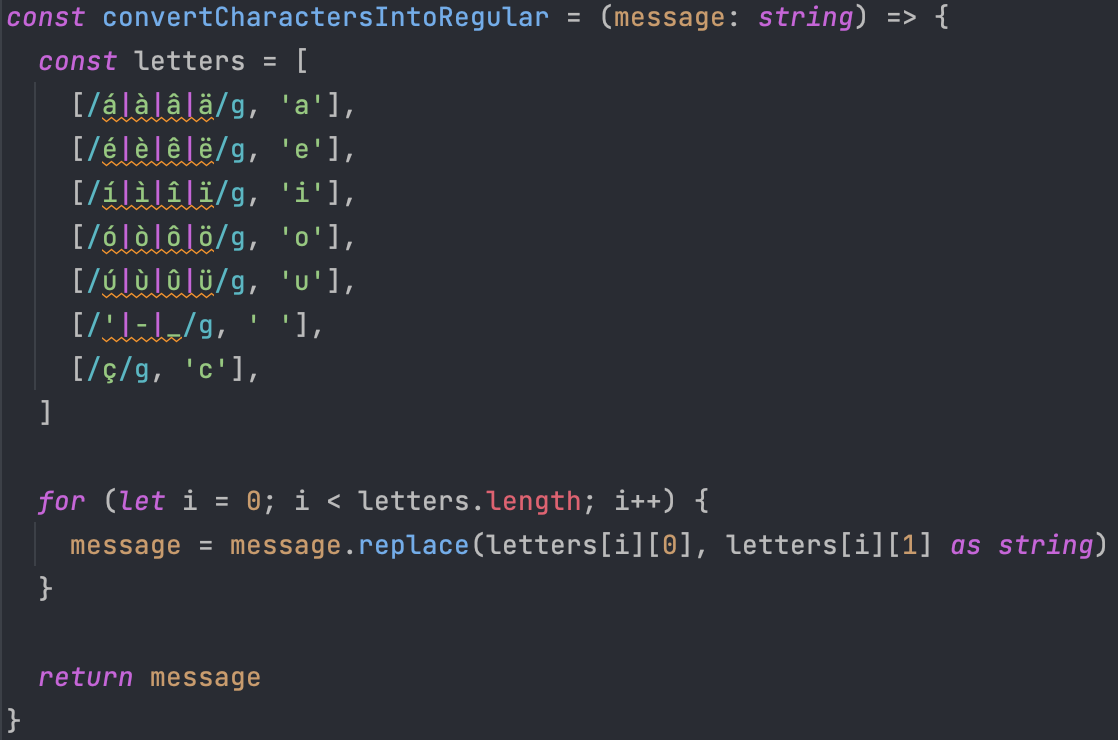
\includegraphics[scale=.6]{assets/fonction-accent.png}
	\caption{Fonction filtre pour les accents}
\end{figure}

\newpage

Cette fonction permet de transformer chaque accent d'une lettre en la lettre elle-même sans accent. Pour ce faire, elle boucle sur la question du joueur pour chaque type d'accent et si elle est présente, il la remplace par celle sans accent. Enfin, elle renvoie le résultat.\newline

Enfin, il reste une notion qui n'a pas été traitée, il s'agit du pluriel. Si un joueur demande "Est-ce que les cartes chance peuvent provoquer une chute ?" ou "Est-ce qu'une carte chance peut provoquer une chute ?", ce n'est pas la même chose pour le bot du au fait que les mots clés qu'il doit repérer peuvent s'écrire différemment selon le pluriel de ce mot.\newline

Afin de palier à ce problème, nous avons décidé d'implémenter une fonction qui ressemble fort à la fonction précédente : 

\begin{figure}[!h]
	\centering
	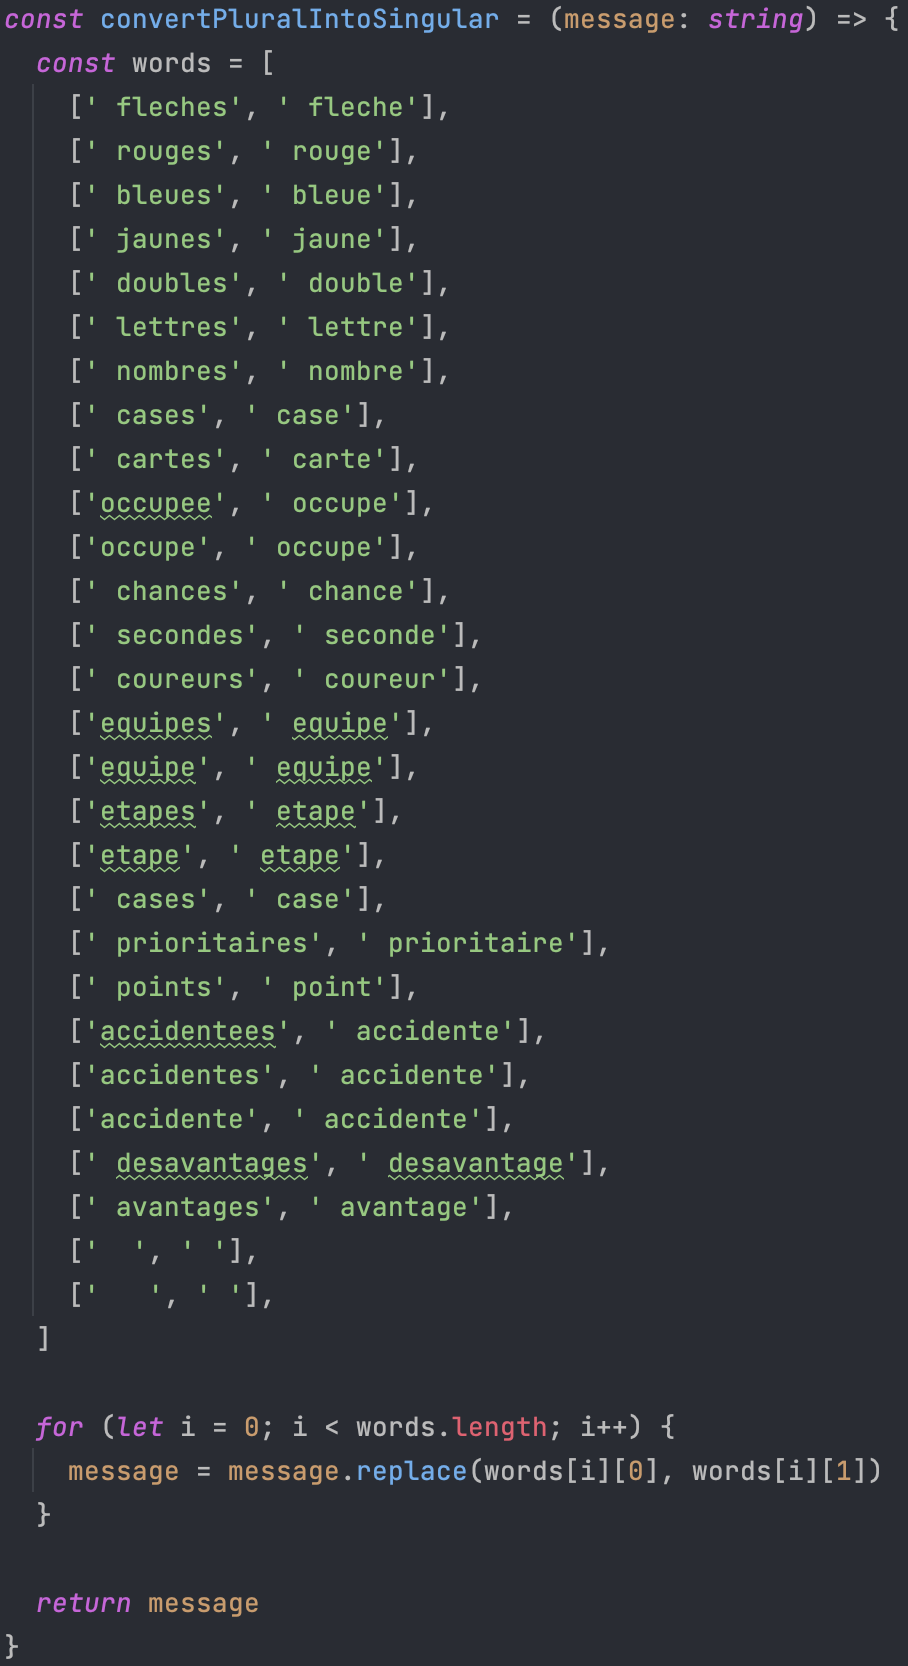
\includegraphics[scale=.6]{assets/fonction-pluriel.png}
	\caption{Fonction filtre pour le pluriel}
\end{figure}

\newpage

Cette fonction permet donc de retirer le pluriel des mots. En effet, le bot a été alimenté par des questions au singulier donc cette fonction retire le pluriel des mots importants s'ils sont au pluriel afin de s'assurer une meilleure tolérance. Cette fonction boucle sur chaque mot de la phrase et quand elle repère un des mots de la liste, le remplace par son équivalent au singulier.\newline

Il faut préciser une petite subtilité de cette fonction. Elle permet également d'isoler les mots auxquels le joueur a oublié l'apostrophe. En effet, si un joueur écrit "detape" ou "d'etape", cette fonction permettra d'isoler le mot "etape" afin de comprendre la phrase même en cas d'oubli d'apostrophe.\newline

Grâce à toutes ces améliorations, le bot comprend les questions avec ou sans accents, au pluriel ou au singulier et avec ou sans apostrophes.

\newpage

\section{Intelligence artificielle adversaire}

\newpage

\section{Interface}

\newpage

\section{Conclusion}

\end{document}